\documentclass[review]{elsarticle}
\usepackage{lineno, hyperref}

%% or use the graphicx package for more complicated commands
%% \usepackage{graphicx}
\graphicspath{{./images/}}

%% The amssymb package provides various useful mathematical symbols
\usepackage{amssymb}

%% The lineno packages adds line numbers. Start line numbering with
%% \begin{linenumbers}, end it with \end{linenumbers}. Or switch it on
%% for the whole article with \linenumbers after \end{frontmatter}.
\usepackage{lineno}

\modulolinenumbers[5]

\journal{Energy and Buildings}

%% `Elsevier LaTeX' style
\bibliographystyle{elsarticle-num}
%%%%%%%%%%%%%%%%%%%%%%%

\begin{document}

\begin{frontmatter}

\title{Building Energy Retrofits Under Capital Constraints\tnoteref{mytitlenote}}
\tnotetext[mytitlenote]{Fully documented methods available \href{https://github.com/buildsci/retrofitLCC}{here}.}

%% Group authors per affiliation:
\author{Matthew Dahlhausen}
\author{Mohammad Heidarinejad}
\author{Jelena Srebric}
\address{University of Maryland}
%%\fnref{myfootnote}
%%\fntext[myfootnote]{Since 1880.}

%% or include affiliations in footnotes:
%%\author[mymainaddress,mysecondaryaddress]{Elsevier Inc}
%%\ead[url]{www.elsevier.com}

%%\author[mysecondaryaddress]{Global Customer Service\corref{mycorrespondingauthor}}
%%\cortext[mycorrespondingauthor]{Corresponding author}
%%\ead{support@elsevier.com}

%%\address[mymainaddress]{1600 John F Kennedy Boulevard, Philadelphia}
%%\address[mysecondaryaddress]{360 Park Avenue South, New York}

\begin{abstract}
Write the abstract last.  4 sentences.  State the problem. Say why it's an interesting problem.  Say what your solution achieves.  Say what follows from your solution.  
\end{abstract}

\begin{keyword}
Office building; energy retrofit; energy efficiency measures; simple payback; staging; integrative design; measure bundles; measure packages; energy simulation 
\end{keyword}

\end{frontmatter}

\linenumbers

\section{Introduction}
Governments and institutions are focusing on building energy efficiency as an area for sizable, cost-effective energy use reduction and greenhouse gas mitigation \cite{McKinsey2009, Farese2012}.  Commercial buildings are important to consider, as they are capital intensive and long-lasting, with a median lifetime of 70 years \cite{BEDB3.2.7}. Without considerable efforts to retrofit the current building stock for energy efficiency, as much as 80\% of 2005 thermal energy consumption can remain past 2050 \cite{Urge-Vorsatz2013141}. Currently, while 86\% of construction costs go to building renovation, little of that goes to improving the energy efficiency of buildings \cite{Wang2012}. Renovation rates are around 2.2\%, with an 11\% average energy savings \cite{Olgyay2010244}. This rate needs to grow several-fold, with average savings around 55\%, to approach modest emission reduction targets and Architecture 2030 goals  \cite{Olgyay2010244}. Few renovation projects in the U.S. have achieved this savings level, with one recent study identifying only 50 such projects, known as deep or advanced energy retrofits \cite{NBI2011, AERG2011}.\par  
Lack of access to capital, insufficient payback, and saving uncertainty are top barriers to making energy retrofits more prevalent \cite{EEI2014, Abadie2012551}.  Most projects are funded with limited internal capital, sometimes with assistance from grants, rebates, and other incentives.  These projects have tended towards individual lighting, controls, and HVAC equipment measures with reliable savings, as it can be very expensive to go through an extensive energy audit that may not significantly reduce the savings uncertainty. While the practice of single measure ranking by simple-payback results in good financial payback on a per-measure basis, it doesn't take advantage of measure integration that can yield greater energy savings. Most notably, heating and cooling load reduction measures enable downsizing central mechanical equipment for significant replacement cost savings.  This means that choosing measure with optimal payback individually may not yield the best retrofit decision overall.  Uncertainty and capital budgets make energy retrofits an economic problem, not just a physical one.\par
Several studies have investigated and established methodologies for choosing energy retrofits, summarized by \cite{Ma2012889}.  A subset of the retrofit literature considers the integrative aspect of measure selection. \cite{Rysanek2013324} show performance of measure packages under different decision criteria and the impact of uncertainty.  This approach captures the interaction between retrofit measures.  However, it is not always possible to implement all measures at once, largely depending on available capital.  \cite{Kumbaroglu2012327} demonstrate a process to implement measures in order depending on capital availability.  This reduces financial risk exposure of a large retrofit project, and stays within an internal budget, but does not consider what measure package would result in the best savings.  Both approaches are needed.  Extending the project timeline incorporates major equipment replacements that are already embedded in capital plans into a comprehensive retrofit package.  This allows targeted load reductions to precede equipment replacement, and to account for the cost of waiting.  There is a trade-off between sacrificing expected life of equipment by replacing it now with other measures, or waiting until end-of-life and forgoing possible energy savings from implementing measures sooner.\par 
This paper establishes a methodology for evaluating energy retrofit packages under capital constraints, demonstrates it through a case-study of an office building in Philadelphia, PA, and discusses the significance of the difference in capital availability to the optimal retrofit decisions.  

\section{Methods}
\textbf{2 pages describing method, 5 pages details} \par
Energy retrofit measure selection is dependent on capital availability, financial criteria, and uncertainties in energy savings and energy costs.  Including measure interaction and savings uncertainties is necessary to properly account for a measure's impact on building performance.  This increases the number of options to consider, and requires energy simulation to handle the complexity of measure interaction.  Installing measures longitudinally based on a fixed capital budget adds further complexity, as the order in which measures are installed becomes significant. Load reduction measures allow equipment downsizing, and there is a performance difference for different size systems with the same energy efficiency  measures.  This greatly increases the number of energy simulation options to consider.
This study constructs all the possible retrofit path-options, including this downsizing difference, to measure the impact of capital constraints on the best retrofit measure option.   Figure \ref{flowchart} shows the process of building path options to consider for a building retrofit under capital constraints.

\begin{figure}[h]
	\centering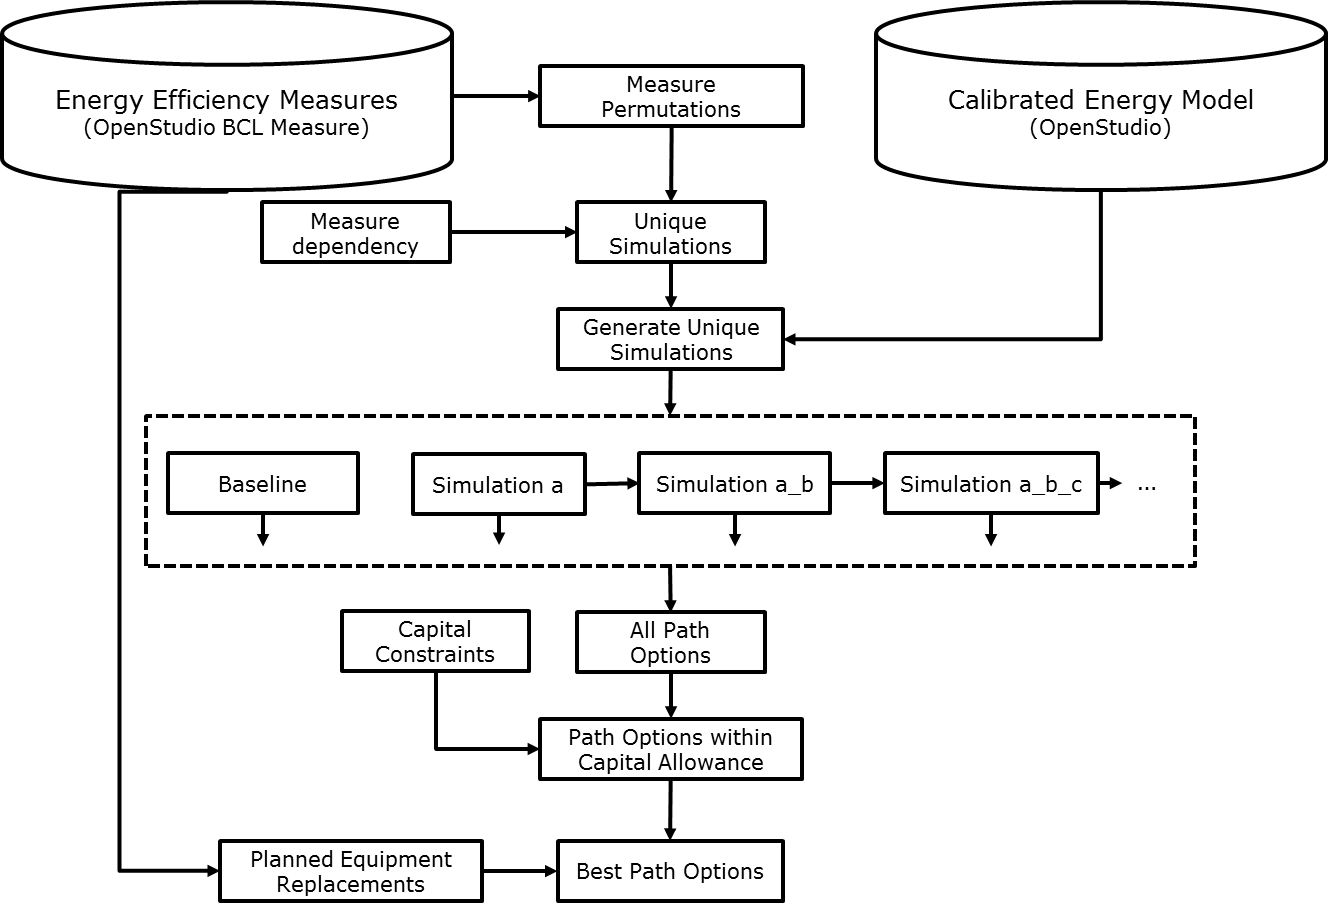
\includegraphics[width=0.8\linewidth]{flowchart.png}
	\caption{Flowchart}
	\label{flowchart}
\end{figure}

\subsection{Case Study}
The case study is a commercial office building at the Philadelphia Navy Yard, shown in Figures \ref{Bldg101a},\ref{Bldg101b}. It was originally built as a barracks, and underwent major renovation in 1999 to become an office building. The building is about 75,000 ft2 (6,968 m2), of which about 60,000 ft2 (5,574 m2) is conditioned space, about 40,000ft2 (3,716 m2) of that office, spread over 3 stories and a conditioned basement. The Energy Utilization Index (EUI) in this study is referenced to conditioned floor area.  The building exterior wall is 1.5ft (0.46m) thick brick, and has a window-to-wall ratio of 17\%.  Three Variable Air Volume (VAV) units with DX cooling serve the building. A gas boiler serves heating coils at each air handler and provides reheat for terminal boxes in each thermal zone. Gas hot water heaters provide service hot water.\par
\begin{figure}[h]
	\centering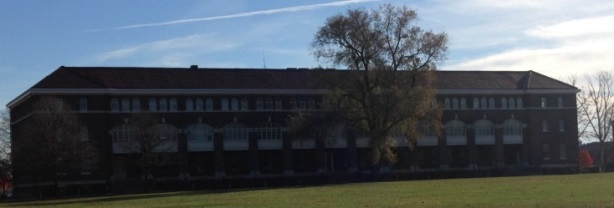
\includegraphics[width=0.4\linewidth]{Bldg101photo.jpg}
	\caption{Figure caption}
	\label{Bldg101a}
\end{figure}
\begin{figure}[h]
	\centering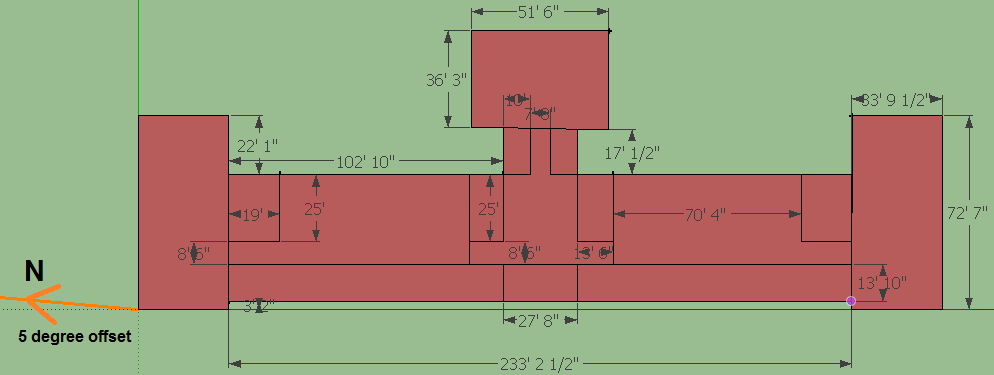
\includegraphics[width=0.4\linewidth]{Bldg101layout.png}
	\caption{Figure caption}
	\label{Bldg101b}
\end{figure}
The building energy model uses the Openstudio\textbf{[REF]} modeling platform.  The simplifications on the model are to assume an identical floor plan on each story, which is nearly the case in the building.  The fenestration is modeled with a set window-to-wall ratio on each exterior wall, rather than modeling each window individually, to improve simulation speed with little accuracy loss on load calculations \cite{Liu2011409}.  Mechanical equipment and lighting specifications are detailed from design drawings.  Plug load is modeled with a set area density for office, conference, and lobby areas from sub-meter data, and equipment schedules were then adjusted to match the hourly plug load profile\cite{Delgoshaei2013, Xu2012}.  Air infiltration is assumed to be a uniform, constant 0.2 ACHnat across the exterior enclosure \textbf{[REF? used 189]}. The model uses AMY weather data from the Philadelphia International Airport, located a few miles from the building site. A detailed summary of building instrumentation and calibration are available in \cite{Dasgupta2012, Dahlhausen2014}.    
The model calibrates to 10-month hourly sub-metered energy data for heating, cooling, service hot water, fan, lighting, total building electric, and total building gas energy use. Plug load and miscellaneous electric use, including water systems pumps and elevators use, is assumed equal to the total building electrical energy use less all other metered electrical loads – cooling, fans, and lighting. January 2012 data are not available, as sub-meter data was not installed until late January, and HVAC sub-meter data in December 2012 are not comparable, as the building underwent a major controls upgrade. The lack of data for these periods increases the uncertainty in heating energy use for model calibration, as nearly a fourth of annual heating degree days occurred in January. The calibration disregards anomalous service hot water use data in April and May, when water use spiked, coinciding with a construction period on the second floor. Table \ref{calibration} shows coefficient of variation of the root square mean error (CVRSME) and normalized mean bias error (NMBE) calibration statistics for each end use following ASHRAE Guideline 14 \cite{ASHRAE14}. The calibrated setpoint temperature was around 72$^{\circ}$F (~22$^{\circ}$C)  with some variation to match observed VAV temperature control.

\begin{table}[h]
	\centering
	\begin{tabular}{l l l l}
		\hline
		& \textbf{CVRSME} & \textbf{NMBE} & \textbf{Months}\\
		\hline
		Calibration Target & 15\% & 5\% & All \\
		All Electricity & 6.1\% & -0.6\% & All \\
		Plug Loads & 5.9\% & -2.1\% & All \\
		Lighting & 4.9\% & 2.6\% & All \\
		Fans & 9.3\% & -1.2\% & Omit December \\
		Cooling & 12.6\% & 3.6\% & Omit December \\
		All Gas & 12.0\% & 2.3\% & Omit December \\
		Heating & 12.6\% & 1.7\% & Omit December \\
		Service Hot Water & 9.5\% & 2.3\% & Omit April and May \\
		\hline
	\end{tabular}
	\caption{Building 101 Energy End Use Calibration Metrics}
	\label{calibration}
\end{table}

\subsubsection{Energy Efficiency Measures}
This study considers seven energy efficiency measures, shown in Table \ref{measures}.  The selected measures were commonly recommended in energy audits of the building.  Costs, shown in Table \ref{measures_cost}, are from RSMeans \cite{RSmeans2014}.

\begin{table}[h]
	\centering
	\begin{tabular}{|p{3cm}|p{8cm}|p{1cm}|}
		\hline
		\textbf{EEM} & \textbf{Description} & \textbf{Source} \\
		\hline
		Exterior Wall Insulation and Finish System & Add an exterior insulation and finish system, with 4" (0.1 m) EPS board, R-16, reduce infiltration by 30\% & - \\
		\hline
		Lighting Power Density Reduction & Reduce conference and office lighting power density from 1.15 to 0.9 W/ft$^2$ (12.38 to 9.69 W/m$^2$) & - \\
		\hline
		Occupancy Sensors & Reduce lighting fraction from 0.2 to 0.05 during unoccupied hours on weekdays, and 0.15 to 0.05 on weekends & - \\
		\hline
		Reduce Infiltration by 15\% & - & - \\
		\hline
		Window Film & Reduce SHGC from 0.764 to 0.38 & - \\
		\hline
		Condensing Boiler Replacement & Replace boiler with 90\% efficient condensing boiler, auto-size capacity and flow rates for loop, lower supply temperature to 140 $^{\circ}$F (60 $^{\circ}$C) & - \\
		\hline
		Condensing Unit Replacement & Replace condensing units with auto-sized unit with high speed EER 11.5 and low speed EER 16.2 & - \\
		\hline
	\end{tabular}
	\caption{Building 101 Energy Efficiency Measures}
	\label{measures}
\end{table}

\begin{table}[h]
	\centering
	\begin{tabular}{l l l}
		\hline
		\textbf{EEM} & \textbf{Cost/Unit} & \textbf{Cost} \\
		\hline
		Exterior Wall Insulation and Finish System & \$4.78/ft$^2$ wall area & \$927,930 \\
		Lighting Power Density Reduction & \$4.78/ft$^2$ floor area & \$202,886\\
		Occupancy Sensors & \$1.06/ft$^2$ floor area & \$44,991 \\
		Reduce Infiltration by 15\% & \$?/ft$^2$ wall area& \$00,000 \\
		Window Film & \$18.93/ft$^2$ glazing & \$182,311 \\
		Condensing Boiler Replacement & \$20,706 + \$4.05/kW & variable \\
		Condensing Unit Replacement & \$7,909 + \$2693.91/kW & variable \\
		\hline
	\end{tabular}
	\caption{Building 101 Energy Efficiency Measures}
	\label{measures_cost}
\end{table}

\subsection{Results}
Show the difference in the solution depending on the capital availability.

\section{Discussion}
\textbf{2 pages comparison to related work}

compare to \cite{Rysanek2013324}

\section{Conclusions}
0.5 pages

\section{\LaTeX\ templates}


\subsection{Lists}
\begin{itemize}
\item Bullet point one
\item Bullet point two
\end{itemize}

\begin{enumerate}
\item Numbered list item one
\item Numbered list item two
\end{enumerate}

\subsection{Equations}
\begin{equation}
\label{eq:emc}
e = mc^2
\end{equation}

\section*{Acknowledgements}
This material is based upon work supported by the Energy Efficient Buildings Hub (EEB Hub), an energy innovation hub sponsored by the U.S. Department of Energy under Award Number DE-EE0004261. The author would like to thank Richard Sweetser for sharing his valuable experience, Payam Delgoshaei for sharing the sub metered energy data for 2012.

\section*{References}
\bibliography{./references/master_ref_list}

\end{document}